%%%%%%%%%%%%%%%%%%%%%%%%%%%%%%%%%%%%%%%%%%%%%%%%%%%%%%%%%%%%%%%
%% OXFORD THESIS TEMPLATE

% Use this template to produce a standard thesis that meets the Oxford University requirements for DPhil submission
%
% Originally by Keith A. Gillow (gillow@maths.ox.ac.uk), 1997
% Modified by Sam Evans (sam@samuelevansresearch.org), 2007
% Modified by John McManigle (john@oxfordechoes.com), 2015
% Modified by Ulrik Lyngs (ulrik.lyngs@cs.ox.ac.uk), 2018-, for use with R Markdown
%
% Ulrik Lyngs, 25 Nov 2018: Following John McManigle, broad permissions are granted to use, modify, and distribute this software
% as specified in the MIT License included in this distribution's LICENSE file.
%
% John commented this file extensively, so read through to see how to use the various options.  Remember that in LaTeX,
% any line starting with a % is NOT executed.

%%%%% PAGE LAYOUT
% The most common choices should be below.  You can also do other things, like replace "a4paper" with "letterpaper", etc.

% 'twoside' formats for two-sided binding (ie left and right pages have mirror margins; blank pages inserted where needed):
%\documentclass[a4paper,twoside]{templates/ociamthesis}
% Specifying nothing formats for one-sided binding (ie left margin > right margin; no extra blank pages):
%\documentclass[a4paper]{ociamthesis}
% 'nobind' formats for PDF output (ie equal margins, no extra blank pages):
%\documentclass[a4paper,nobind]{templates/ociamthesis}

% As you can see from the line below, oxforddown uses the a4paper size, 
% and passes in the binding option from the YAML header in index.Rmd:
\documentclass[a4paper, nobind]{templates/ociamthesis}


%%%%% ADDING LATEX PACKAGES
% add hyperref package with options from YAML %
\usepackage[pdfpagelabels]{hyperref}
% handle long urls
\usepackage{xurl}
% change the default coloring of links to something sensible
\usepackage{xcolor}

\definecolor{mylinkcolor}{RGB}{0,0,139}
\definecolor{myurlcolor}{RGB}{0,0,139}
\definecolor{mycitecolor}{RGB}{0,33,71}

\hypersetup{
  hidelinks,
  colorlinks,
  linktocpage=true,
  linkcolor=mylinkcolor,
  urlcolor=myurlcolor,
  citecolor=mycitecolor
}


% add float package to allow manual control of figure positioning %
\usepackage{float}

% enable strikethrough
\usepackage[normalem]{ulem}

% use soul package for correction highlighting
\usepackage{color, soulutf8}
\definecolor{correctioncolor}{HTML}{CCCCFF}
\sethlcolor{correctioncolor}
\newcommand{\ctext}[3][RGB]{%
  \begingroup
  \definecolor{hlcolor}{#1}{#2}\sethlcolor{hlcolor}%
  \hl{#3}%
  \endgroup
}
% stop soul from freaking out when it sees citation commands
\soulregister\ref7
\soulregister\cite7
\soulregister\citet7
\soulregister\autocite7
\soulregister\textcite7
\soulregister\pageref7

%%%%% FIXING / ADDING THINGS THAT'S SPECIAL TO R MARKDOWN'S USE OF LATEX TEMPLATES
% pandoc puts lists in 'tightlist' command when no space between bullet points in Rmd file,
% so we add this command to the template
\providecommand{\tightlist}{%
  \setlength{\itemsep}{0pt}\setlength{\parskip}{0pt}}
 
% allow us to include code blocks in shaded environments

% User-included things with header_includes or in_header will appear here
% kableExtra packages will appear here if you use library(kableExtra)
\usepackage{booktabs}
\usepackage{longtable}
\usepackage{array}
\usepackage{multirow}
\usepackage{wrapfig}
\usepackage{float}
\usepackage{colortbl}
\usepackage{pdflscape}
\usepackage{tabu}
\usepackage{threeparttable}
\usepackage{threeparttablex}
\usepackage[normalem]{ulem}
\usepackage{makecell}
\usepackage{xcolor}


%UL set section header spacing
\usepackage{titlesec}
% 
\titlespacing\subsubsection{0pt}{24pt plus 4pt minus 2pt}{0pt plus 2pt minus 2pt}


%UL set whitespace around verbatim environments
\usepackage{etoolbox}
\makeatletter
\preto{\@verbatim}{\topsep=0pt \partopsep=0pt }
\makeatother


%%%%%%% PAGE HEADERS AND FOOTERS %%%%%%%%%
\usepackage{fancyhdr}
\setlength{\headheight}{15pt}
\fancyhf{} % clear the header and footers
\pagestyle{fancy}
\renewcommand{\chaptermark}[1]{\markboth{\thechapter. #1}{\thechapter. #1}}
\renewcommand{\sectionmark}[1]{\markright{\thesection. #1}} 
\renewcommand{\headrulewidth}{0pt}





% UL page number position 
\fancyfoot[C]{\emph{\thepage}} %regular pages
\fancypagestyle{plain}{\fancyhf{}\fancyfoot[C]{\emph{\thepage}}} %chapter pages




%%%%% SELECT YOUR DRAFT OPTIONS
% This adds a "DRAFT" footer to every normal page.  (The first page of each chapter is not a "normal" page.)

% IP feb 2021: option to include line numbers in PDF

% for line wrapping in code blocks
\usepackage{fancyvrb}
\usepackage{fvextra}
\DefineVerbatimEnvironment{Highlighting}{Verbatim}{breaklines=true, breakanywhere=true, commandchars=\\\{\}}

% This highlights (in blue) corrections marked with (for words) \mccorrect{blah} or (for whole
% paragraphs) \begin{mccorrection} . . . \end{mccorrection}.  This can be useful for sending a PDF of
% your corrected thesis to your examiners for review.  Turn it off, and the blue disappears.


%%%%% BIBLIOGRAPHY SETUP
% Note that your bibliography will require some tweaking depending on your department, preferred format, etc.
% If you've not used LaTeX before, I recommend just using pandoc for citations -- this is what's used unless you specific e.g. "citation_package: natbib" in index.Rmd
% If you're already a LaTeX pro and are used to natbib or something, modify as necessary.

% this allows the latex template to handle pandoc citations




% Uncomment this if you want equation numbers per section (2.3.12), instead of per chapter (2.18):
%\numberwithin{equation}{subsection}


%%%%% THESIS / TITLE PAGE INFORMATION
% Everybody needs to complete the following:




% Master's candidates who require the alternate title page (with candidate number and word count)
% must also un-comment and complete the following three lines:

% Uncomment the following line if your degree also includes exams (eg most masters):
%\renewcommand{\submittedtext}{Submitted in partial completion of the}
% Your full degree name.  (But remember that DPhils aren't "in" anything.  They're just DPhils.)


% Term and year of submission, or date if your board requires (eg most masters)



%%%%% YOUR OWN PERSONAL MACROS
% This is a good place to dump your own LaTeX macros as they come up.

% To make text superscripts shortcuts
\renewcommand{\th}{\textsuperscript{th}} % ex: I won 4\th place
\newcommand{\nd}{\textsuperscript{nd}}
\renewcommand{\st}{\textsuperscript{st}}
\newcommand{\rd}{\textsuperscript{rd}}

%%%%% THE ACTUAL DOCUMENT STARTS HERE
\begin{document}

%%%%% CHOOSE YOUR LINE SPACING HERE
% This is the official option.  Use it for your submission copy and library copy:
\setlength{\textbaselineskip}{22pt plus2pt}
% This is closer spacing (about 1.5-spaced) that you might prefer for your personal copies:
%\setlength{\textbaselineskip}{18pt plus2pt minus1pt}

% You can set the spacing here for the roman-numbered pages (acknowledgements, table of contents, etc.)
\setlength{\frontmatterbaselineskip}{17pt plus1pt minus1pt}

% UL: You can set the line and paragraph spacing here for the separate abstract page to be handed in to Examination schools
\setlength{\abstractseparatelineskip}{13pt plus1pt minus1pt}
\setlength{\abstractseparateparskip}{0pt plus 1pt}

% UL: You can set the general paragraph spacing here - I've set it to 2pt (was 0) so
% it's less claustrophobic
\setlength{\parskip}{2pt plus 1pt}

%
% Customise title page
%
\def\crest{}
\renewcommand{\university}{}
\renewcommand{\submittedtext}{}
\renewcommand{\thesistitlesize}{\fontsize{22pt}{28pt}\selectfont}
\renewcommand{\gapbeforecrest}{25mm}
\renewcommand{\gapaftercrest}{25mm
}


% Leave this line alone; it gets things started for the real document.
\setlength{\baselineskip}{\textbaselineskip}


%%%%% CHOOSE YOUR SECTION NUMBERING DEPTH HERE
% You have two choices.  First, how far down are sections numbered?  (Below that, they're named but
% don't get numbers.)  Second, what level of section appears in the table of contents?  These don't have
% to match: you can have numbered sections that don't show up in the ToC, or unnumbered sections that
% do.  Throughout, 0 = chapter; 1 = section; 2 = subsection; 3 = subsubsection, 4 = paragraph...

% The level that gets a number:
\setcounter{secnumdepth}{2}
% The level that shows up in the ToC:
\setcounter{tocdepth}{1}


%%%%% ABSTRACT SEPARATE
% This is used to create the separate, one-page abstract that you are required to hand into the Exam
% Schools.  You can comment it out to generate a PDF for printing or whatnot.

% JEM: Pages are roman numbered from here, though page numbers are invisible until ToC.  This is in
% keeping with most typesetting conventions.
\begin{romanpages}

% Title page is created here

%%%%% DEDICATION

%%%%% ACKNOWLEDGEMENTS


%%%%% ABSTRACT


%%%%% MINI TABLES
% This lays the groundwork for per-chapter, mini tables of contents.  Comment the following line
% (and remove \minitoc from the chapter files) if you don't want this.  Un-comment either of the
% next two lines if you want a per-chapter list of figures or tables.
\dominitoc % include a mini table of contents

% This aligns the bottom of the text of each page.  It generally makes things look better.
\flushbottom

% This is where the whole-document ToC appears:


% Uncomment to generate a list of tables:
%%%%% LIST OF ABBREVIATIONS
% This example includes a list of abbreviations.  Look at text/abbreviations.tex to see how that file is
% formatted.  The template can handle any kind of list though, so this might be a good place for a
% glossary, etc.

% The Roman pages, like the Roman Empire, must come to its inevitable close.
\end{romanpages}

%%%%% CHAPTERS
% Add or remove any chapters you'd like here, by file name (excluding '.tex'):
\flushbottom

% all your chapters and appendices will appear here
{word count 2789/2598}

\hypertarget{research-approach}{%
\chapter{Research Approach}\label{research-approach}}

\hypertarget{methodological-considerations}{%
\subsection*{Methodological considerations}\label{methodological-considerations}}
\addcontentsline{toc}{subsection}{Methodological considerations}

Social semiotics are inherently subjective and situated (Kress, 2011, p36), which is congruent with my philosophical approach of constructivist ontology and interpretivist epistemology. Social semiotics approaches are iterative, so `description', `analysis' and `interpretation' are not distinct stages of the research process (Bezemer and Mavers, 2011, p196). The core of the methods used are informed by the works on multimodal communication analysis produced by Norris (2004; 2009), Kress (2011), Bezemer and Mavers (2011), and Cowan (2014). These authors are/were (socio-)linguistic experts in the education field. However, their works are adaptable to the political science context, and proved invaluable for analysing multimodal communication.

My mixed-methods research design is complex and carefully considered. There are four analytical chapters: \textbf{Chapter Four: Statistical Analysis} of key variables to assess the dataset and set up further analysis; \textbf{Chapter Five: Individual Timeline Trends Analysis} pairing interactive quantitative timeline visualisations with inductive qualitative thematic analysis to explore each actor's use of gastropopulism; \textbf{Chapter Six: Nationalism and Class} uses deductive qualitative thematic analysis to examine how the central themes of extant gastropopulism research manifest in my sample and theory; \textbf{Chapter Seven: Performative Eating} develops an original framework, Multimodal Social Semiotics Timeline Transcription (MMSSTT), to analyse performative eating videos. This dissertation's structure will produce breadth and depth of analysis of multimodal gastropopulist performances.

\hypertarget{sample}{%
\subsection*{Sample}\label{sample}}
\addcontentsline{toc}{subsection}{Sample}

The population of my study is multimodal content of British and American political actors associated with populist performances using food as a communicative mode. The political actors selected for my sample are: Alexandria Ocasio-Cortez (USA, left-wing); Donald Trump (USA, right-wing); Jeremy Corbyn (UK, left-wing); Nigel Farage (UK, right-wing). Farage and AOC were named in Garcia-Santamaria's (2020, p146) concluding remarks about other political actors who use food to connect to audiences. The addition of Trump and Corbyn enables analysis of how gastropopulism is performed within and across ideologies and countries. This is an important element to empirically test the impact of conflating of (gastro)populism with ideology and/or region. I next briefly contextualise the selected actors' celebrity origins.

AOC represents New York's 14th Congressional District, population \textasciitilde700,000, yet she has 8.5 million Instagram followers (ocasio-cortez.house.gov, \emph{n.d.}). Her `everyday influencer' celebrity role attracts a large social media audience through ``carefully crafted and stylised'' interactive and multimodal politainment centring relatability and `ordinariness' (Starita and Trillò, 2022, p334; Rasulo, 2020, p125). She frequently self-presents idealised gastropopulist performances of her personal role through `stories' and livestreams, which disappear after 24 hours, aligning with Moffitt's (2016, p85) concern that the celebrity role may enable political actors to avoid scrutiny and accountability. This resonates with `disappearing' gastropopulist performances, as the aura of spontaneity and `personal' content may be used to disguise explicitly political messages.

In 2023, the active and crucial part Trump's Apprentice role played in his public identity during his 2016 campaign is easily forgotten; he planned to work on season eight until June 2015, when the network publicly cut ties due to Trump's ``derogatory statements'' at campaign rallies about Mexican immigrants (St.~James, 2015). Though his reality star celebrity origins were filtered through traditional broadcast media, he quickly adapted this to harness the affordances of social media platforms, particularly Twitter (McDonnell and Wheeler, 2019, p430). Furthermore, his adversarial `billionaire boss' reality star role fostered parasocial illusions and inherently blurred the line of perceived (in)authenticity regarding his political role and politics, mutually reinforcing his celebrity and politician roles (Street, 2019, pp7-8).

Farage and Corbyn's political careers long pre-date social media (and `populism' becoming a buzzword), so their public identities were largely filtered through traditional media. As such, their celebrity politician origins are rooted in their `politics', inclusive of style and substance (Street, 2019, p10; Moffitt, 2016, p85). Moffitt (2016, p84) states that a ``key tactic'' for populists relying on traditional media is brazen opportunism with media appearances, ``particularly those that ostensibly bring them closer to `the people'\,''.

As an MEP for a minor party --- both elements of which inspire little media attention --- Farage courted press coverage to establish his identity through extensive gastropopulist performances, frequently involved holding a pint of beer (Tindall, 2022, p135). Farage leveraged the traditional media and asserted the political relevance of euroscepticism, and over decades of work, significantly contributed to shifting the UK's political landscape (Hart and Winter, 2022, p38).

In contrast, the `celebrity politician' role was seemingly given to, rather than sought by Corbyn. Corbyn was a highly rebellious but relatively unknown backbench Labour MP for 32 years before his shock landslide victory in Labour's 2015 leadership contest (Quinn, 2016, p765). However, his performed (or perhaps more accurately, \emph{perceived}) authenticity and radical-left policies were extremely popular with young people, dubbed `Corbynmania' (Quinn, 2016, p764). Given his long-established reticence to blend his personal and politician roles (Hattenstone, 2015), the unanticipated addition of a `celebrity' role perhaps posed a challenge for Corbyn's impression management strategies.

Ultimately, influenced by Street (2019), considering the \emph{celebrity} origin and affordances of the selected actors' identities has been highly insightful for my analysis of gastropopulism, particularly when explaining the variations, motivations, and credibility of individuals' performances. My dissertation is neither a critique nor defence of `celebrity' in politics, but it asserts the explanatory and cultural power of celebrity and popular culture in UK and US contexts.

\hypertarget{data}{%
\subsection*{Data}\label{data}}
\addcontentsline{toc}{subsection}{Data}

The unit of analysis is the post, always constituted of visual and/or audiovisual content, and often containing textual content (e.g., captions). As my approach stresses \emph{multimodal} communication, purely textual content was excluded. My data collection approach was guided by the existing empirical gastropopulism studies, starting with \emph{manual} scraping of each actor's \emph{entire} official Instagram account {[} \emph{my adjustments italicised}{]} (Garcia-Santamaria, 2020, p130; Starita, 2022, p94; Demuru, 2021, p511). Akin to Demuru, I extended my data collection through Internet searches of ``{[}actor{]} + {[}food/eating/cooking{]}''. My data consists of public communications from political figures collected from verified official sources. Where visible, I censored comments from non-verified users. Accordingly, my dissertation raises no particular ethical concerns. The following tables present descriptive statistics for each actor's Instagram accounts {[}Table 3.1{]} and the makeup of my sample {[}Table 3.2{]}. My final sample was n=163 {[}excluding 15 non-gastropopulist performances, addressed shortly{]}.

\begin{table}

\caption{\label{tab:unnamed-chunk-1}Actors’ Instagram statistics [03/07/2023]}
\centering
\begin{tabular}[t]{l|l|l|l|l}
\hline
Actor & Handle & Follower Count & Post Count & Date Joined\\
\hline
AOC & \textbackslash{}@AOC & 8,500,000 & 577 & 01/2012\\
\hline
Trump & \textbackslash{}@realdonaltrump & 23,400,000 & 6,126 & 04/2013\\
\hline
Corbyn & \textbackslash{}@jeremycorbyn & 511,000 & 1,519 & 04/2016\\
\hline
Farage & \textbackslash{}@nigel\_farage & 180,000 & 432 & 03/2017\\
\hline
\end{tabular}
\end{table}

\begin{table}

\caption{\label{tab:unnamed-chunk-2}Descriptive statistics for the sample}
\centering
\fontsize{14}{16}\selectfont
\begin{tabu} to \linewidth {>{\raggedright}X>{\centering}X>{\centering}X>{\centering}X>{\centering}X>{\centering}X}
\hline
\multicolumn{1}{c|}{ } & \multicolumn{4}{c|}{\textbf{Actor}} & \multicolumn{1}{c}{ } \\
\cline{2-5}
\textbf{Variable} & \makecell[c]{\textbf{AOC}\ \ \\ N = 26 \\[+0]} & \makecell[c]{\textbf{Corbyn}\ \ \\ N = 45 \\[+2]} & \makecell[c]{\textbf{Farage}\ \ \\ N = 65 \\[+3]} & \makecell[c]{\textbf{Trump}\ \ \\ N = 27 \\[+10]} & \makecell[c]{\textbf{Overall}\ \ \\ N = 163 \\[+15]}\\
\hline
Gastropopulism &  &  &  &  & \\
\hline
\hspace{1em}Gastropopulism & 26\ \ (100\%) & 45\ \ (96\%) & 65\ \ (96\%) & 27\ \ (73\%) & 163\ \ (92\%)\\
\hline
\hspace{1em}Not Gastropopulism & 0\ \ (0\%) & 2\ \ (4.3\%) & 3\ \ (4.4\%) & 10\ \ (27\%) & 15\ \ (8.4\%)\\
\hline
Data Format &  &  &  &  & \\
\hline
\hspace{1em}Audiovisual & 13\ \ (50\%) & 11\ \ (24\%) & 10\ \ (15\%) & 14\ \ (52\%) & 48\ \ (29\%)\\
\hline
\hspace{1em}Visual & 13\ \ (50\%) & 34\ \ (76\%) & 55\ \ (85\%) & 13\ \ (48\%) & 115\ \ (71\%)\\
\hline
Platform &  &  &  &  & \\
\hline
\hspace{1em}Instagram & 21\ \ (81\%) & 39\ \ (87\%) & 54\ \ (83\%) & 14\ \ (52\%) & 128\ \ (79\%)\\
\hline
\hspace{1em}Other & 0\ \ (0\%) & 0\ \ (0\%) & 4\ \ (6.2\%) & 3\ \ (11\%) & 7\ \ (4.3\%)\\
\hline
\hspace{1em}Twitter & 2\ \ (7.7\%) & 2\ \ (4.4\%) & 0\ \ (0\%) & 4\ \ (15\%) & 8\ \ (4.9\%)\\
\hline
\hspace{1em}YouTube & 3\ \ (12\%) & 4\ \ (8.9\%) & 7\ \ (11\%) & 6\ \ (22\%) & 20\ \ (12\%)\\
\hline
Distribution &  &  &  &  & \\
\hline
\hspace{1em}Actor's social media & 24\ \ (92\%) & 40\ \ (89\%) & 55\ \ (85\%) & 9\ \ (33\%) & 128\ \ (79\%)\\
\hline
\hspace{1em}Mass media organisation & 1\ \ (3.8\%) & 2\ \ (4.4\%) & 7\ \ (11\%) & 10\ \ (37\%) & 20\ \ (12\%)\\
\hline
\hspace{1em}Other social media & 1\ \ (3.8\%) & 3\ \ (6.7\%) & 3\ \ (4.6\%) & 8\ \ (30\%) & 15\ \ (9.2\%)\\
\hline
\end{tabu}
\end{table}

These descriptive tables establish differences within my sample concerning how each actor uses social media and food in their political communications. Table 3.2 shows that 79\% of my sample was collected from Instagram, and (coincidentally) 79\% was collected from the actors' official social media accounts. I next lay out the structure of my methods and analysis, including my gastropopulism codebook.

\hypertarget{methods-and-analysis}{%
\section{Methods and Analysis}\label{methods-and-analysis}}

The structure of my methods, analysis, and findings is complex but cohesive. I created an extensive coding frame with variables informed by academic literature, and coded my entire gastropopulism sample {[}n=163{]}. During the initial data collection, `non-gastropopulist' performances were informally flagged {[}n=15{]} and not coded further. My detailed codebook can be found in {Appendix A} {only include important variables}. For conceptual clarity, I now provide an extract of the codebook regarding gastropopulism. Briefly, I used this to individually code the features of gastropopulism as `present' or `absent', and items coded as `not gastropopulism' were excluded from the sample. To properly examine the multimodality of the features of gastropopulism, each mode was coded ``in terms specific to its affordances {[}and shaping{]}, and in terms shared by all modes'' (Kress, 2011, p38). Multimodal approaches identify/interpret meanings through ``common parlance'' or theoretical accounts (Kress, 2011, p39).

\begin{figure}
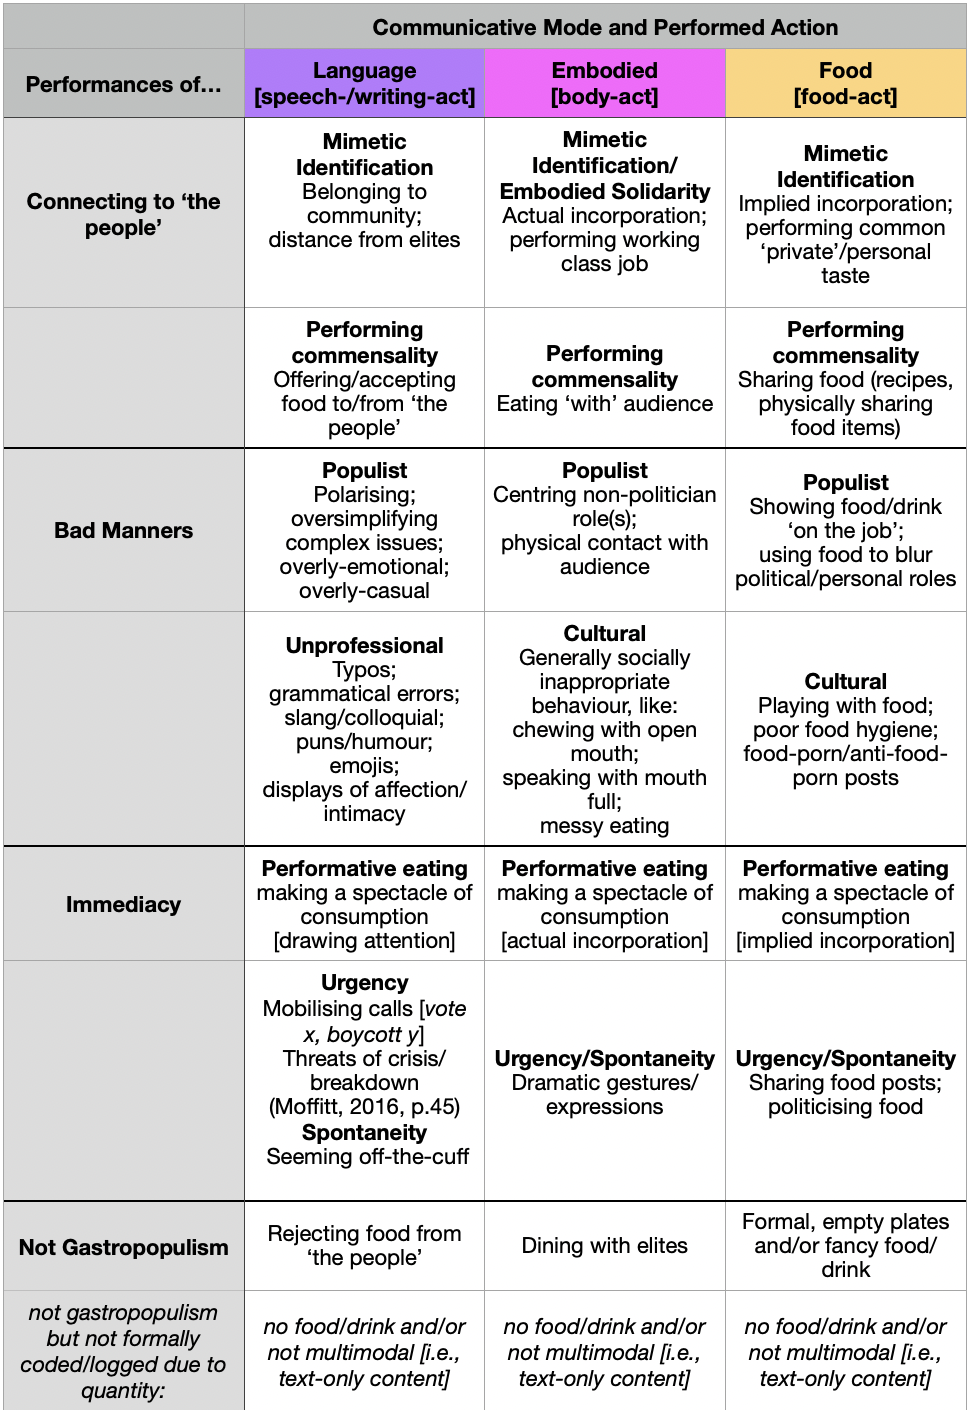
\includegraphics[width=13.44in]{../oxforddown-3.5/DissdataIMAGES/gpcode} \caption{Codebook extract, Gastropopulism}\label{fig:unnamed-chunk-3}
\end{figure}

During the coding process, I generated informal notes of ``potential data items of interest, questions, connections between data items, and other preliminary ideas'' (Kiger and Varpio, 2020, p850). As a result, themes became clearer and I clarified my codes accordingly, congruent with my iterative social semiotics approach (Bezemer and Mavers, 2011, p196). Each argument is developed through analysis of one or more relevant items, screenshots of which are presented using the \texttt{knitr} (Xie, 2023) and \texttt{gridextra} (Auguie, 2022) R packages. The process of selecting items for deeper analysis was informed by ``analytical and rhetorical purposes'', that is, ``telling'' moments with strong potential for analytical insights (Bezemer and Mavers, 2011, pp194-195). The performative eating chapter analyses only audiovisual data, the other chapters draw from both visual and audiovisual data.

\hypertarget{statistical-analysis}{%
\subsection*{Statistical Analysis}\label{statistical-analysis}}
\addcontentsline{toc}{subsection}{Statistical Analysis}

The statistical analysis chapter assesses how gastropopulist performances are constructed. I adapted Starita's (2022, p95) approach to generate a summary statistics table of my entire sample using my coding of key variables and the \texttt{gtsummary} R package (Sjoberg, 2021). `Key variables' were informed by the literature, and guide my further analysis. The table quantitatively explores the dataset's distribution, showing the count and relative frequency of selected categories per actor, ideology, region, and overall. This structure is a considered effort to empirically test performative, ideological, and regional theories regarding gastropopulism.

Key variables:
* Incorporation: whether the food was eaten
* Cultural association: how the food relates to the actor's cultural identity
* Nourishment: healthy, moderate, unhealthy
* Taste: flavour profile
* Individual features of gastropopulism
* Individual Trends

The statistical analysis chapter establishes how political actors construct their gastropopulist performances. Subsequent chapters continue this work, through examining how political actors use \emph{multimodal} gastropopulism performances to construct their \emph{public identities}.

\hypertarget{mixed-methods-individual-timeline-thematic-analysis}{%
\subsection*{Mixed-methods Individual Timeline Thematic Analysis}\label{mixed-methods-individual-timeline-thematic-analysis}}
\addcontentsline{toc}{subsection}{Mixed-methods Individual Timeline Thematic Analysis}

This chapter quantitatively and qualitatively examines each actor's entire data in the sample, through timeline visualisations paired with inductive qualitative thematic analysis. The \texttt{vistime} (Raabe, 2022), \texttt{plotly} (Sievert, 2020) and \texttt{emoji} (Hvitfeldt, 2022) R packages were used to generate individual interactive quantitative timeline visualisations. This original design aims to visualise potential patterns in each actor's use of gastropopulism, such as clusters during campaign periods.

The following visualisation of the entire dataset introduces the interactive elements. Hovering on markers displays the date posted and sample ID (Px indicating image, Vx indicating video, and on Trump's individual timeline, NGx indicating non-gastropopulist content). Datapoints are colour coded to reflect whether the individual theme was present, implied, or absent (N/A {[}pre-slogan{]} are coloured grey for Corbyn). On the individual timelines, datapoints used for further analysis are overlaid with symbols, hovering displays the sample ID, date and food. Furthermore, relevant election dates are marked with flag emojis, hovering over which displays the election type and date.

\begin{figure}
\centering
\includegraphics{03-ResearchApproach_files/figure-latex/unnamed-chunk-4-1.pdf}
\caption{\label{fig:unnamed-chunk-4}Full Dataset Timeline Visualisation}
\end{figure}

When generating the individual visualisations, Trump's data raised some methodological challenges, due to: his over \textbf{two year ban from Meta} (Instagram and FaceBook) platforms {[}06/01/2020-07/02/2023{]} after inciting a deadly insurrection attempt (Meta, 2021); the \textbf{10 non-gastropopulist items}, eight of ostentatious empty plates at elite political events; and as shown in Table 3.2, the \textbf{distribution of his gastropopulist content} being fairly evenly split between his own social media accounts {[}n=9{]}, his senior advisor Jason Miller's official Twitter and Instagram accounts (both @JasonMillerinDC) {[}n=8{]}, and mass media organisations {[}n=10{]}.

Accordingly, Trump's individual timeline marks non-gastropopulist items with grey crosses, and his Meta ban as a grey line. Furthermore, the y axis uses the \texttt{Distribution} variable to delineate between data collected from: his own social media; Miller's social media; mass media. Trump's non-gastropopulist items are marked for transparency because they represent a quarter (n=10, 27\%) of his initial data collected (n=37), and my argument is based on the purposeful alignment of his gastropopulism with his campaigns. Thus, the timings of his non-gastropopulist performances are relevant, though not further analysed.

Non-gastropopulist items were excluded from other actors' timelines, as no such items were coded for AOC, only two for Corbyn (4.5\%) and three for Farage (4.3\%). Additionally, the other actors' data were primarily collected from their own social media accounts (AOC 92\%; Corbyn 89\%; Farage 86\%), so their y axes do not use the \texttt{distribution} variable. Four items dated between 2011-2014 were excluded from Farage's timeline as they distorted the visualisation's scale {[}P3, 09/09/2011; V13, 03/05/2013; P120, 23/04/2014, used in §6.2 Class; V16, 03/10/2014, used in §7 Performative Eating{]}. For Corbyn, four items occurred pre-slogan so are colour-coded grey on his timeline {[}P2; P36; P41; P44{]}. Documenting these methodological decisions is vital for transparency and replicability (Bezemer and Mavers, 2011, p204).

Each actor's timeline visualisation is followed by a discussion of their individual trend, generated through inductive qualitative thematic analysis. Inductive thematic analysis is highly suited to my social semiotics approach, as it centres the context and data of each actor to develop themes. This chapter allows us to get a sense of how each actor tailors gastropopulism to their needs.

\hypertarget{deductive-qualitative-thematic-analysis}{%
\subsection*{Deductive Qualitative Thematic Analysis}\label{deductive-qualitative-thematic-analysis}}
\addcontentsline{toc}{subsection}{Deductive Qualitative Thematic Analysis}

My deductive qualitative thematic analysis examines how the central themes (nationalism and class) of extant gastropopulism literature manifest within my sample and under my theory. As the aforementioned studies present gastropopulism as a right-wing discursive ideology used to convey exclusionary nationalism, my nationalism analysis considers four instances of exclusionary and inclusionary nationalism by Farage and Trump. The studies also assert gastropopulism as a right-wing tool to convey class belonging, however, this is common to populists across the ideological spectrum (Tindall, 2022, p139). Thus, instead of centring ideology, my analysis scrutinises how the actors' performances of class belonging are shaped by their celebrity and professional roles. This extends the discussions of their individual trends by considering how the actors attempt impression management.

This deductive qualitative thematic analysis chapter aims to build upon existing gastropopulism theory to provide a comprehensive account of gastropopulism that is not distorted by ideological assumptions. Instead, this centres the analytical focus on the actor's integration of communicative modes in their gastropopulist performances, as well as the role of their constructed identity. This chapter offers insights into the performative nature of gastropopulism, and how actors benefit from cohesive gastropopulist performances.

\hypertarget{multimodal-social-semiotics-timeline-transcription}{%
\subsection*{Multimodal Social Semiotics Timeline Transcription}\label{multimodal-social-semiotics-timeline-transcription}}
\addcontentsline{toc}{subsection}{Multimodal Social Semiotics Timeline Transcription}

The final analytical chapter dissects the \emph{multimodality} of gastropopulist performances through examining performative eating videos. This considers the communicative power of political actors publicly demonstrating \emph{you are what you eat} (Diehl, 2017, p12; Bourdieu, 1984, p190; Stano, 2015, p657). The works regarding online eating performers by Hai-Jew (2022) and Rüdiger (2021) were helpful not only to consider the affordances of the audiovisual format in this context, but to scrutinise the inherently performative nature of eating for an audience. Though not written for the political context, they are keenly relevant to my work, owing to their explorations of performed authenticity, intimacy, and spontaneity, as well as the sociocultural role of food and eating.

This chapter is shaped by Norris' (2009, p351) seminal work on multimodal (inter)action analysis, which facilitates analysis of how individual communicative modes interact with each other to convey a single message. ELAN (2023) video annotation software was used to generate multimodal social semiotics timeline transcriptions (MMSSTT). My design adapted Cowan's (2014, pp15-16) multimodal timeline transcript structure (which primarily coded body language modes non-linguistically, using symbols) to incorporate multimodal social semiotics analysis research by Kress (2011) and Bezemer and Mavers (2011). Figure 3.3 below presents my pilot MMSSTT:

\begin{figure}
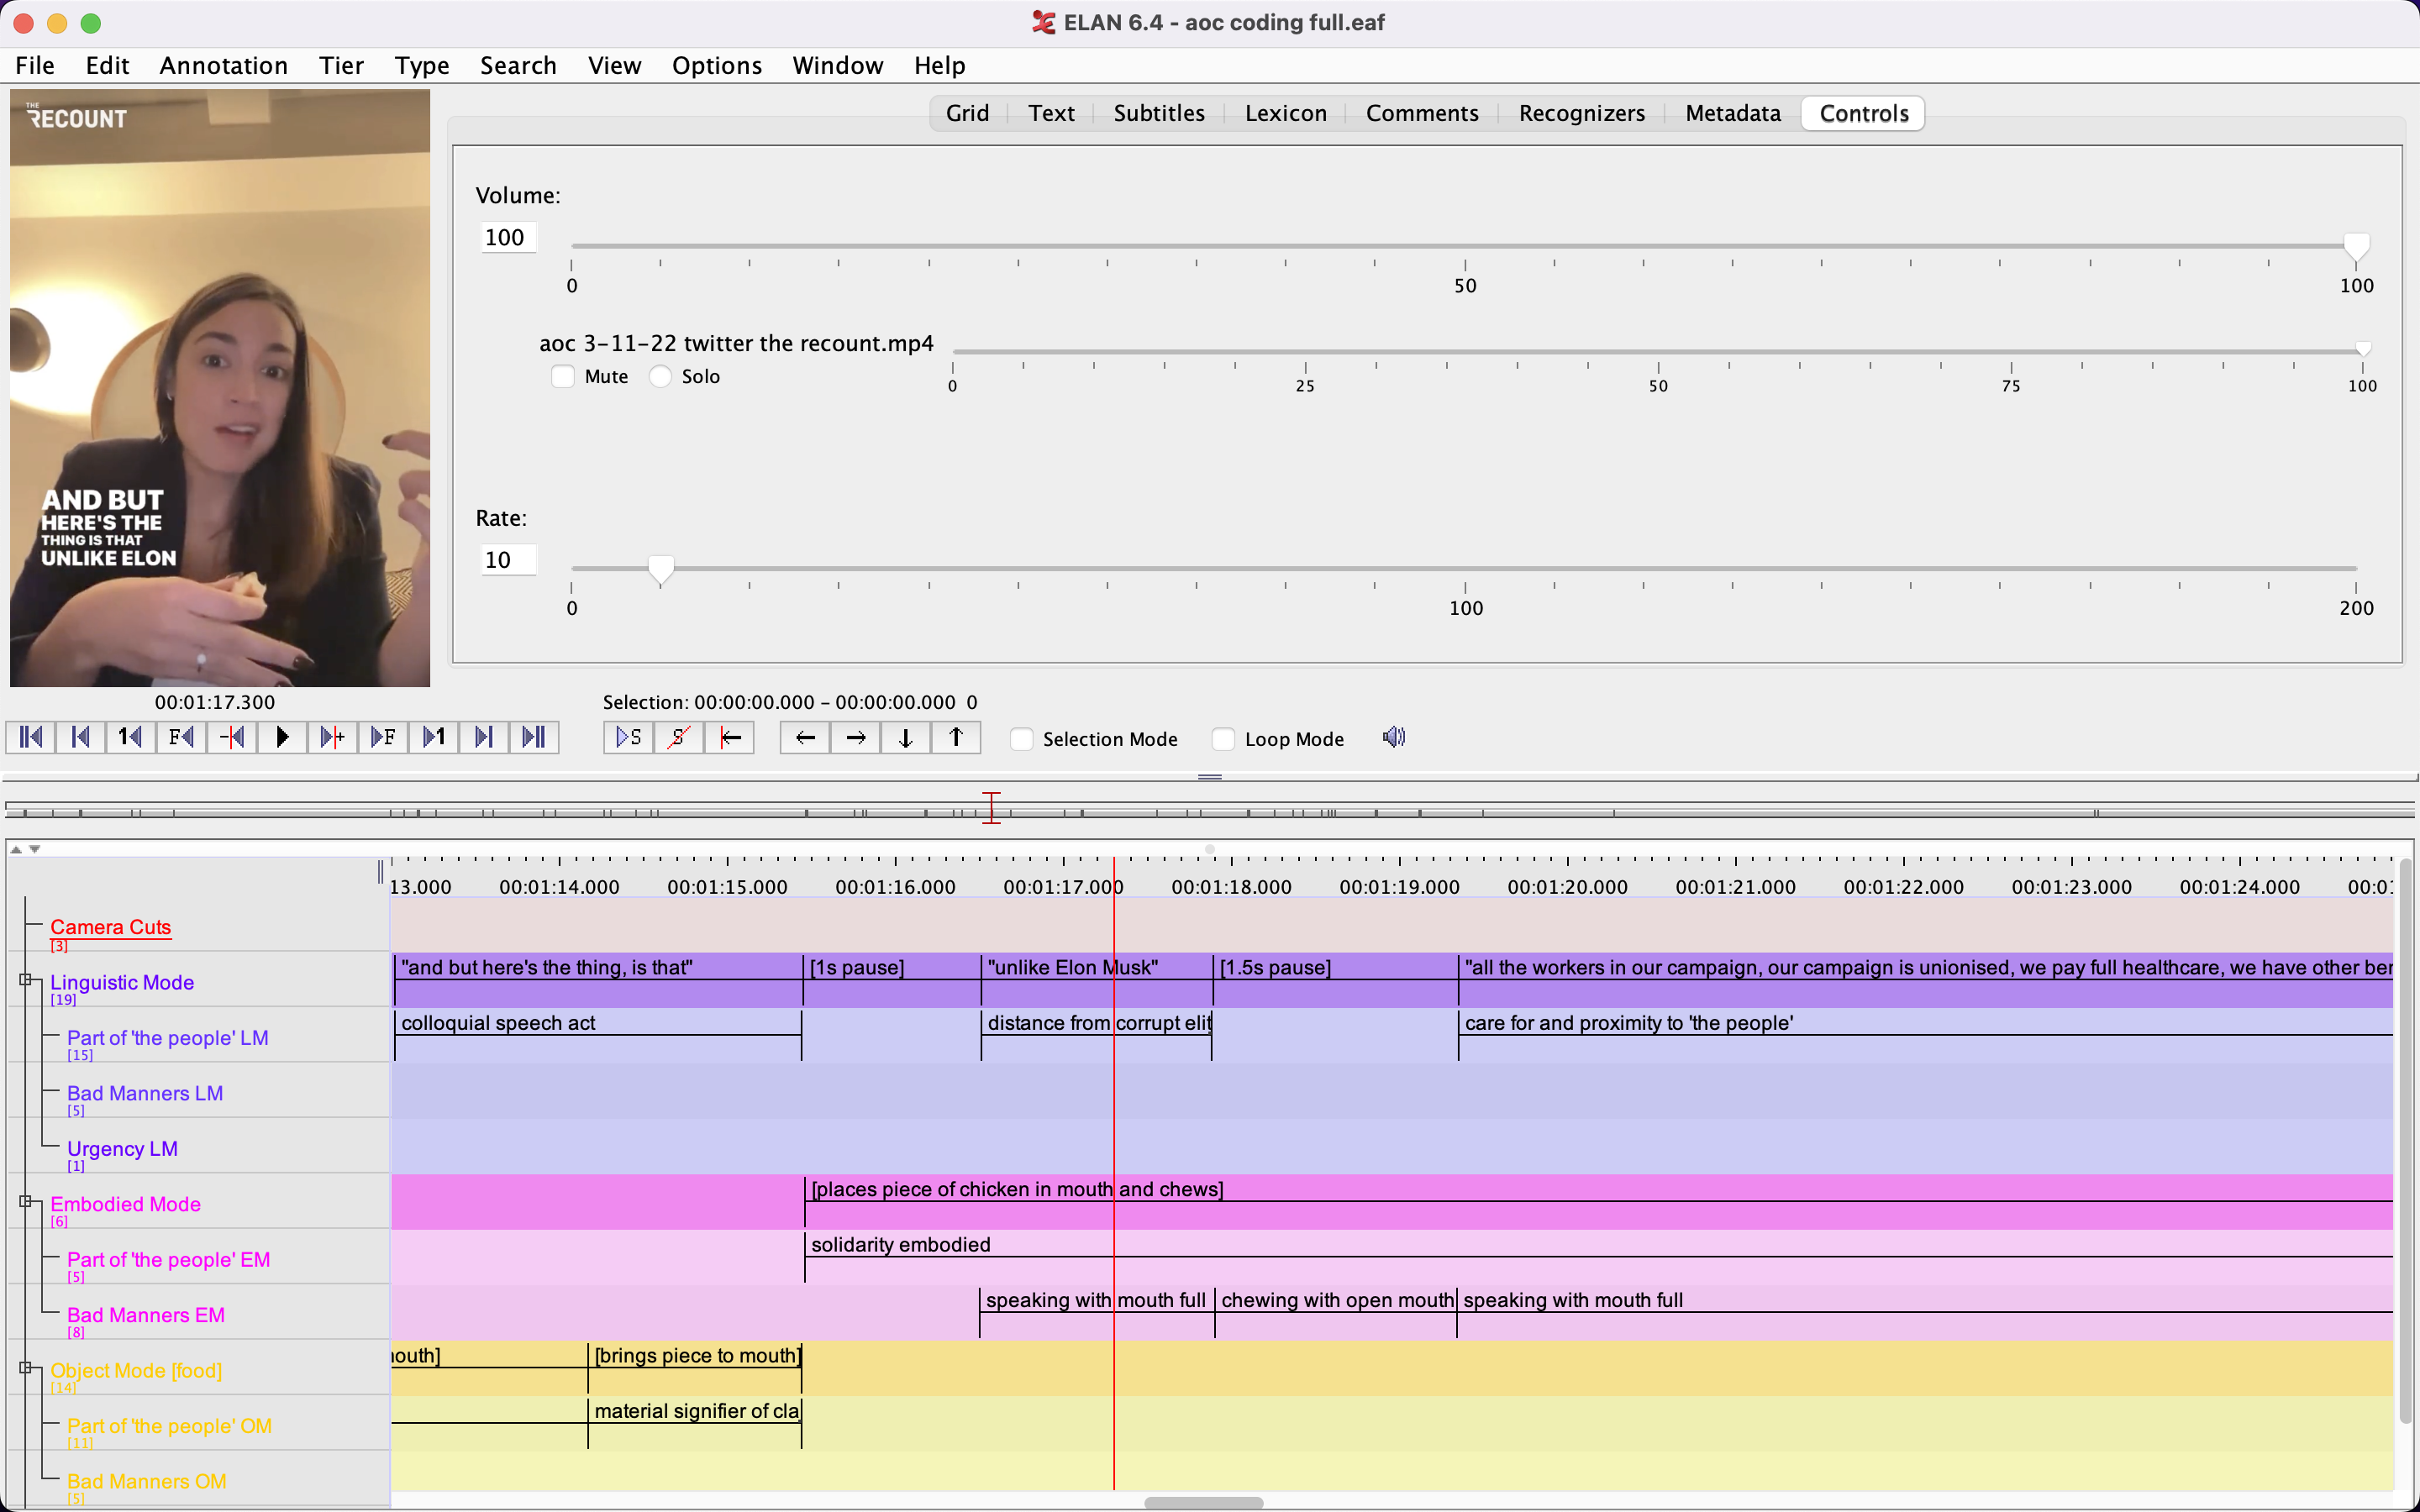
\includegraphics[width=40in]{../oxforddown-3.5/DissdataIMAGES/AOCpilot} \caption{Multimodal social semiotics timeline transcript [pilot]}\label{fig:unnamed-chunk-5}
\end{figure}

Using my gastropopulism codebook, each communicative mode (language, embodied, food) was individually assessed for each feature of gastropopulism (part of `the people', bad manners, immediacy) to conduct granular analysis. Figure 3.3 was conducted before the formal codes were finalised (Bezemer and Mavers, 2011, p195). In the textual analysis, timestamps denote minute:second {[}e.g., 1:17{]}. The layout is structured to illustrate the ``complexities of meaning making'' (Bezemer and Mavers, 2011, p202). This chapter examines how individual communicative modes are choreographed and integrated to build a `natural' and cohesive performance of the features of gastropopulism. This pays particular attention to the communicative power of eating. This analytical method draws from literature across multiple disciplines to develop a useful original design.

\hypertarget{methodology-discussion}{%
\section*{Methodology Discussion}\label{methodology-discussion}}
\addcontentsline{toc}{section}{Methodology Discussion}

Though undeniably complex, this research design is formulated to provide a rigorous and comprehensive account of gastropopulism with robust empirical evidence. Each analytical chapter builds from the previous to form an unprecedented breadth and depth of gastropopulism analysis. Ultimately, this will enable a robust answer to my research question, \emph{how do political actors use multimodal gastropopulist performances to construct and legitimise their public identities?}.

%%%%% REFERENCES


\end{document}
